\documentclass[11pt,a4paper]{article}

\usepackage{fontspec}
\usepackage[russian]{babel}
\setmainfont{cmunrm.otf}[BoldFont=cmunbx.otf,ItalicFont=cmunti.otf,BoldItalicFont=cmunbi.otf]
\setsansfont{cmunss.otf}[BoldFont=cmunsx.otf,ItalicFont=cmunsi.otf,BoldItalicFont=cmunso.otf]
\setmonofont{cmuntt.otf}[BoldFont=cmuntb.otf,ItalicFont=cmunit.otf,BoldItalicFont=cmuntx.otf]

\usepackage[left=20mm,right=15mm,top=18mm,bottom=20mm]{geometry}
\usepackage{amsmath}
\usepackage{graphicx}
\usepackage{float}
\usepackage{xcolor}
\usepackage{booktabs}
\usepackage{tabularx}
\usepackage{array}
\usepackage{listings}
\usepackage[most]{tcolorbox}
\usepackage[labelsep=period,font=small,skip=3pt,justification=raggedright,singlelinecheck=true]{caption}
\usepackage{enumitem}
\usepackage{xurl}
\usepackage[hidelinks,pdfauthor={Тищенко П. В.},pdftitle={Отказоустойчивость координатора MapReduce средствами Apache ZooKeeper}]{hyperref}

\definecolor{accent}{HTML}{2F5D9C}
\definecolor{ok}{HTML}{1E7A45}
\definecolor{bad}{HTML}{B3261E}
\definecolor{codebg}{HTML}{F4F5F8}
\definecolor{cmt}{HTML}{6B7280}

\setlength{\parindent}{1cm}
\setlength{\emergencystretch}{3em}
\setlist{itemsep=1pt,topsep=3pt}
\renewcommand{\arraystretch}{1.15}
\newcolumntype{L}{>{\raggedright\arraybackslash}X}
\setlength{\abovecaptionskip}{3pt}
\setlength{\intextsep}{6pt}
\renewcommand{\topfraction}{0.9}
\renewcommand{\bottomfraction}{0.8}
\renewcommand{\textfraction}{0.07}
\renewcommand{\floatpagefraction}{0.85}
\makeatletter
\@secpenalty=0
\makeatother

\lstset{
  basicstyle=\ttfamily\scriptsize,
  columns=fixed,
  basewidth=0.525em,
  keepspaces=true,
  breaklines=true,
  backgroundcolor=\color{codebg},
  frame=leftline,
  rulecolor=\color{accent},
  framerule=1.5pt,
  xleftmargin=6pt,
  framexleftmargin=4pt,
  aboveskip=4pt,
  belowskip=6pt,
  showstringspaces=false,
  extendedchars=true,
  moredelim=[is][\color{bad}\bfseries]{@@}{@@},
  moredelim=[is][\color{ok}\bfseries]{++}{++},
  moredelim=[is][\color{cmt}]{~~}{~~}
}

\newcommand{\code}[1]{\texttt{#1}}
\newtcolorbox{keybox}{enhanced,colback=accent!6,colframe=accent,boxrule=0.6pt,arc=0pt,left=5pt,right=5pt,top=3pt,bottom=3pt,before upper={\setlength{\parindent}{0pt}}}


\begin{document}

\begin{titlepage}
  \centering
  \vspace*{15mm}
  {\large Домашнее задание №\,4\par}
  {\large «Обеспечение отказоустойчивости средствами Apache ZooKeeper»\par}
  \vspace{40mm}
  {\LARGE\bfseries Ансамбль ZooKeeper и запасной\\[4pt] координатор MapReduce\par}
  \vspace{8mm}
  {\normalsize Выборы лидера, чекпоинт, эпоха и защита записи результата\\ Расчёт пар навыков PHP-вакансий из ДЗ\,3\par}
  \vfill
  \begin{flushright}
    \begin{tabular}{@{}l@{}}
      Выполнил: \textbf{Тищенко Павел Валерьевич}\\
      Группа ИИИ-3-ИнжДан-1-1 (J3310), №\,16\\
      Репозиторий: \url{https://github.com/paulhowever/vk_data_eng_2026_ai_67_tischenko}
    \end{tabular}
  \end{flushright}
  \vspace{25mm}
  {2026\par}
\end{titlepage}


\section{Стенд и конфигурация}

\begin{table}[H]
\centering
\small
\caption{Стенд}
\begin{tabularx}{\linewidth}{@{}lL@{}}
\toprule
Машина & Apple M5, 10 ядер, 16 ГБ RAM, macOS; Docker Engine 29.2.0; Python 3.13, uv \\
Java & локально OpenJDK 17.0.19 (Homebrew), \code{JAVA\_HOME=/opt/homebrew/opt/openjdk@17/libexec/openjdk.jdk/Contents/Home}; в образе Temurin 17.0.20.1, \code{JAVA\_HOME=/opt/java/openjdk} \\
ZooKeeper & 3.9.6, официальный образ \code{zookeeper:3.9.6}, три контейнера \code{hh-zk1..3} (\code{zookeeper/compose.yaml}) \\
Клиент & kazoo 2.11.0, строка подключения \code{127.0.0.1:2181,127.0.0.1:2182,127.0.0.1:2183}, тайм-аут сессии 10\,с \\
Данные & RustFS из ДЗ\,3 (\code{localhost:19000}), объект \code{raw/it\_vacancies\_2024.csv}, эталон \code{results/mapreduce/k2.csv} \\
\bottomrule
\end{tabularx}
\end{table}

Версии взяты из \code{hw4/outputs/stage1\_java.txt}. Вместо трёх распакованных копий дистрибутива я поднял три сервера в Docker. Каждому из репозитория монтируется свой \code{zoo.cfg} и свой \code{myid}. Строки \code{server.N} у всех одинаковые, а \code{clientPort} и \code{dataDir} свои. Контейнер выполняет штатную команду \code{zkServer.sh start-foreground}, PID\,1 в нём --- \code{QuorumPeerMain /conf/zoo.cfg} (\code{stage2\_roles.txt}).
\begin{lstlisting}
$ cat zookeeper/zk2/conf/zoo.cfg                    ~~# zk1, zk3 отличаются только dataDir и clientPort~~
tickTime=2000
initLimit=10
syncLimit=5
dataDir=/zk/zk2/data
clientPort=2182
quorumListenOnAllIPs=true
admin.enableServer=false
4lw.commands.whitelist=srvr,stat,mntr,ruok,cons
server.1=zk1:2888:3888
server.2=zk2:2889:3889
server.3=zk3:2890:3890
\end{lstlisting}

Три строки в конфиге добавлены сверх минимума. С параметром \code{quorumListenOnAllIPs=true} сервер слушает порты кворума и выборов на всех интерфейсах контейнера, а не только на адресе, в который резолвится его собственное имя из \code{server.N}. Параметр \code{admin.enableServer=false} выключает встроенный HTTP AdminServer: он мне не нужен и по умолчанию занимает порт 8080. Через \code{4lw.commands.whitelist} я разрешил четырёхбуквенные команды, которыми смотрю состояние серверов: \code{srvr}, \code{stat}, \code{mntr}, \code{ruok} и \code{cons}. Порты кворума и выборов у серверов разные (2888/3888, 2889/3889, 2890/3890), хотя у каждого контейнера свой IP и хватило бы одной пары. Так конфиги совпадают с тем, что пришлось бы написать для трёх копий на одной машине.

\section{Ансамбль из трёх серверов}

Все шаги выполняет \code{zookeeper/stage2.sh}, выводы лежат в \code{hw4/outputs/stage2\_*.txt}. Я запускал его сразу после \code{docker compose up -d}, поэтому сначала скрипт ждёт, пока все три сервера начнут отвечать \code{Mode: leader} или \code{Mode: follower}. Без этого первые выборы ещё идут, лидер не найден, и остановка «лидера» превращается в \code{docker compose stop} с пустым именем.

\begin{itemize}
  \item \textbf{Роли.} Лидер --- zk3, а zk1 и zk2 --- последователи, это видно по \code{zkServer.sh status}. Команда \code{srvr} показывает у последователей \code{Zxid: 0xb000000ea}, а у лидера \code{0xc00000000}. Старшие 32 бита zxid --- номер эпохи лидера. Новый лидер начал эпоху 0xc, но ни одной транзакции в ней ещё не было, а последователи показывают последнюю запись прошлой эпохи.
  \item \textbf{Минус один.} Остановил лидера zk3 командой \code{docker compose stop}. Скрипт опрашивает \code{zkServer.sh status} и увидел нового лидера zk2 не позже чем через 1,0\,с после начала остановки. Точнее видно по журналу самого ZooKeeper (строки \code{LEADER ELECTION TOOK} на рис.~\ref{fig:ensemble}): выборы заняли 214\,мс у zk2, ставшего лидером, и 204\,мс у zk1. Запись \code{create /minus1} через zk1 прошла и читается через zk2: два сервера из трёх --- это большинство.
  \item \textbf{Минус два.} Остановил ещё и zk2. Процесс zk1 жив (\code{ruok} отвечает \code{imok}), но запросы он не обслуживает. На \code{srvr} сервер отвечает «This ZooKeeper instance is not currently serving requests», а \code{zkServer.sh status} пишет «Error contacting service». И чтение \code{get /minus1}, и запись \code{create /minus2 x} падают с \code{ConnectionLoss}, код выхода \code{zkCli} 1. Один сервер из трёх кворума не образует.
  \item \textbf{Возврат.} Запустил zk3 и zk2: все три снова работают (лидер zk2), и узел \code{/minus1}, записанный без zk3, читается и через zk3.
\end{itemize}

Почему ансамбль переизбрал лидера за доли секунды, а координатору в этапах 3--4 нужно около 12\,с? Команда \code{docker compose stop} --- мягкая остановка: Java-процесс получает SIGTERM, завершается и закрывает свои TCP-соединения. Последователи сразу видят, что связь с лидером пропала, и начинают выборы. Мой замороженный координатор ничего не закрывает, его соединения формально живы, и сервер ждёт, пока истечёт тайм-аут сессии. Лидером стал именно zk2, потому что при выборах голоса сравниваются по последнему zxid, а при равном zxid побеждает больший \code{myid}. У zk1 и zk2 zxid совпадал, и у zk2 номер больше. Выводы этапа собраны на рис.~\ref{fig:ensemble}.

\begin{figure}[!tb]
  \centering
  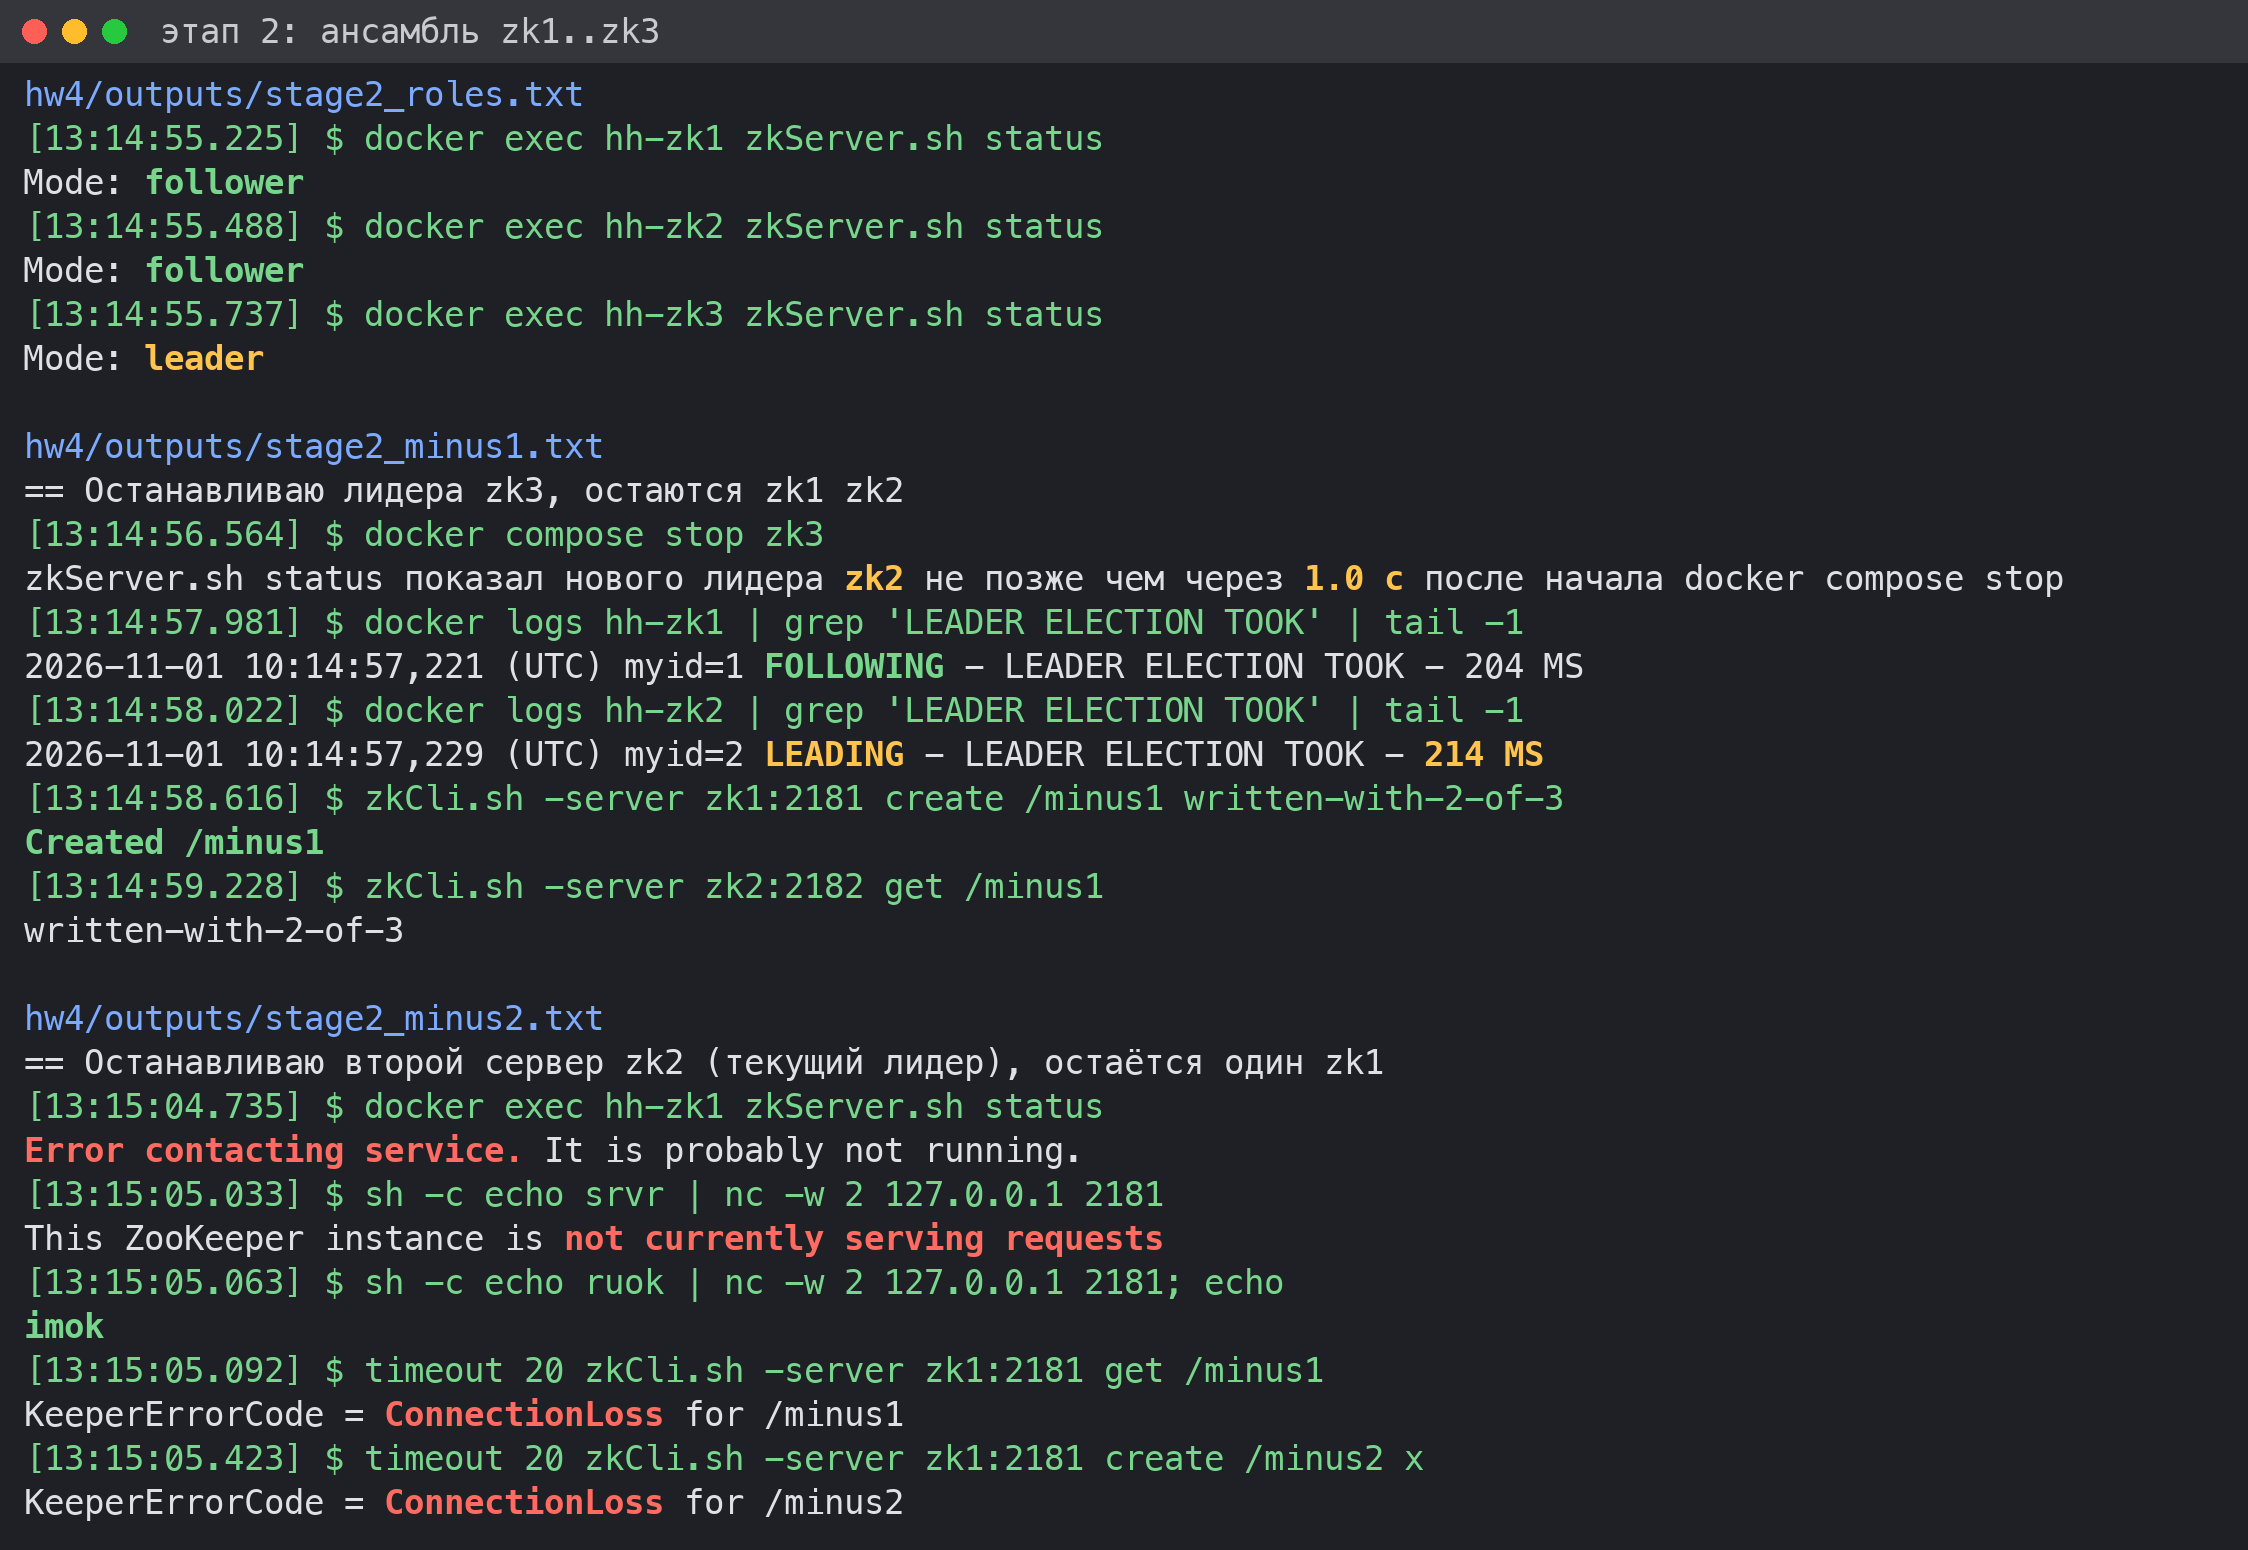
\includegraphics[width=\linewidth]{img/ensemble.png}
  \caption{Роли, остановка одного и двух серверов (фрагмент вывода \code{hw4/outputs/stage2\_*.txt}, строки отобраны, команды и строки журнала ZK сокращены)}
  \label{fig:ensemble}
\end{figure}

\textbf{Эфемерный узел.} «Окно 2» --- это интерактивный \code{zkCli.sh} в отдельном контейнере \code{hh-zk-window2}, подключённый к zk2. Скрипт печатает каждую команду, которую отправляет в это окно, поэтому в выводе видно \code{окно 2> create -e /demo/eph "owned-by-window-2"}. Из «окна 1» \code{stat} показывает \code{ephemeralOwner = 0x2000000cc080001}, это сессия окна 2. Её согласованный тайм-аут я снял командой \code{cons} на zk2: \code{to=30000}, то есть 30\,с (значение \code{zkCli} по умолчанию). Окно я «закрыл» командой \code{docker kill}: клиент умер, не закрыв сессию, как при закрытии терминала. Дальше скрипт раз в $\approx$0,12\,с опрашивает \code{mntr} на zk1. Счётчик \code{zk\_ephemerals\_count} стал 0 не позже чем через 29,8\,с после начала \code{docker kill}. Это чуть меньше 30\,с, потому что тайм-аут отсчитывается от последнего пакета клиента, который был до \code{kill}, а сервер проверяет истечение по границам \code{tickTime} = 2\,с. После этого \code{ls /demo} возвращает \code{[]}, а \code{stat /demo/eph} --- \code{Node does not exist} (рис.~\ref{fig:ephemeral}).

\begin{figure}[!tb]
  \centering
  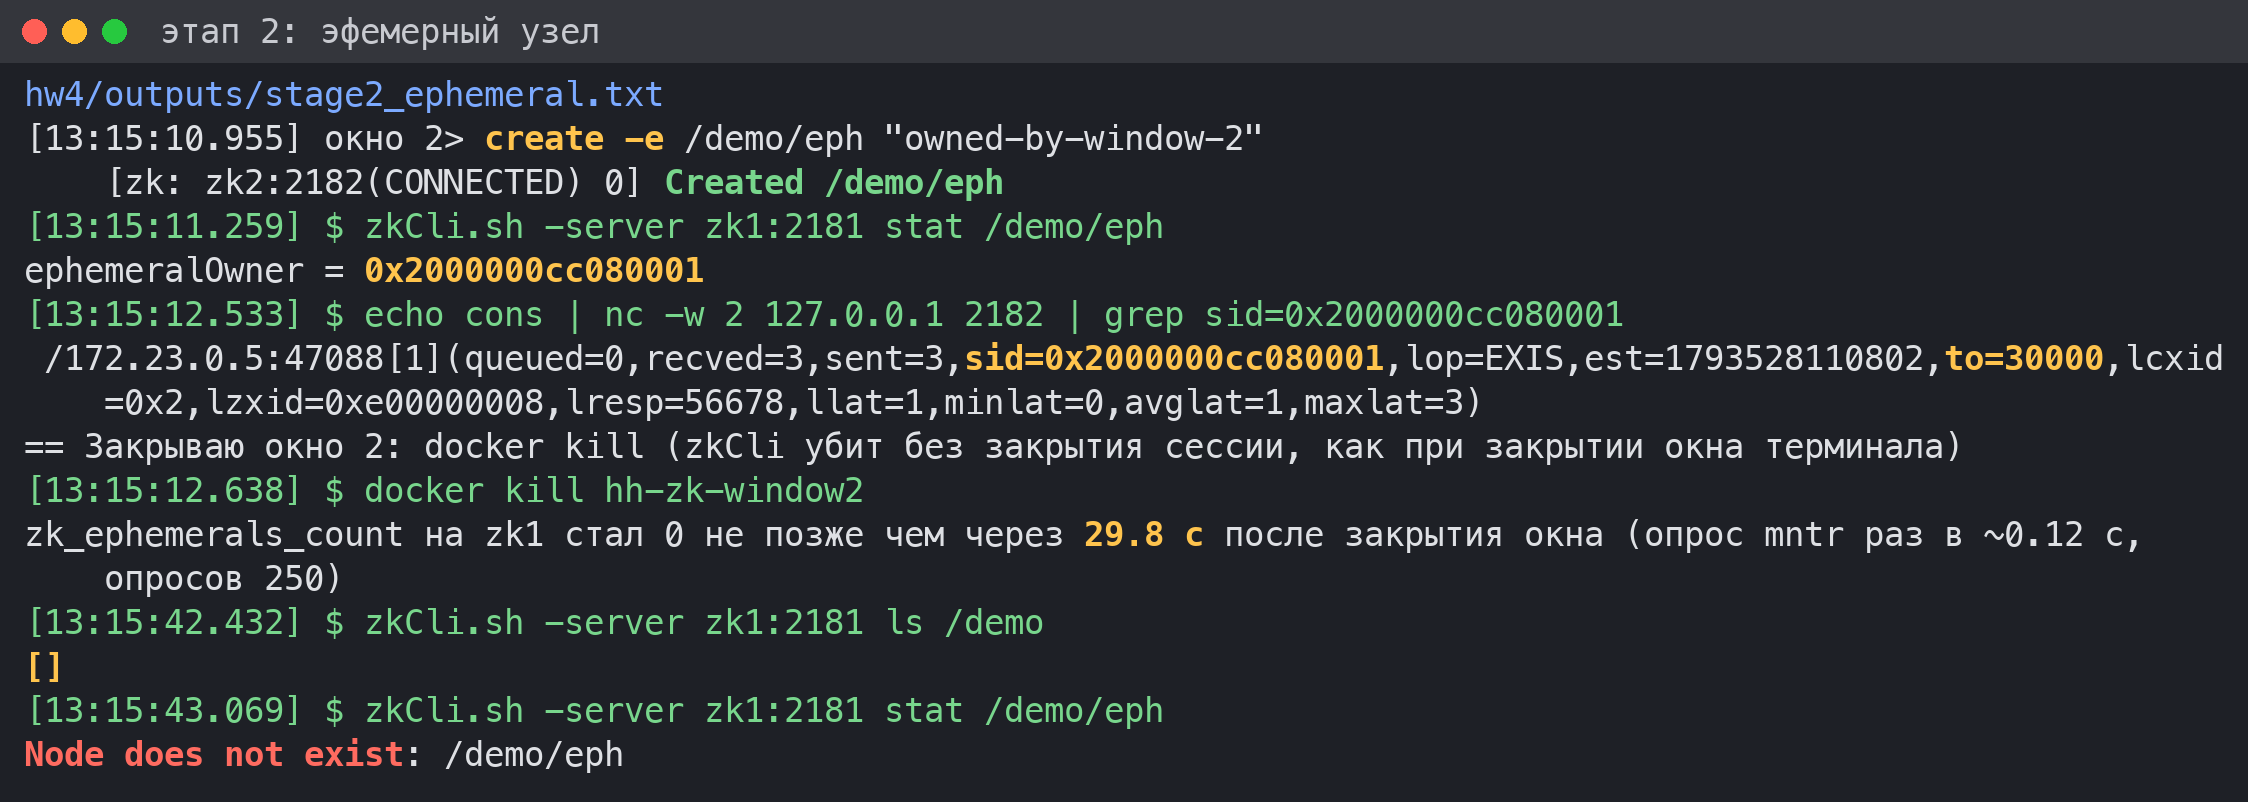
\includegraphics[width=\linewidth]{img/ephemeral.png}
  \caption{Эфемерный узел исчезает после смерти сессии-владельца (фрагмент вывода \code{hw4/outputs/stage2\_ephemeral.txt}, строки отобраны)}
  \label{fig:ephemeral}
\end{figure}

\section{Координатор с запасным}

Пакет \code{hhlake.zk} работает поверх движка ДЗ\,3: нарезка \code{split.plan} (26 чанков по 32\,МиБ), map-функция \code{engine.run\_map}, shuffle в S3, \code{jobs.merge\_blob} и \code{jobs.render\_csv}. Считаются пары навыков ($k=2$). Узлы ZooKeeper лежат под \code{/hhlake/<сценарий>/}.
\begin{itemize}
  \item \textbf{Выборы.} Каждая копия создаёт в \code{election} эфемерный последовательный узел с именем \code{<uuid>-n\_<номер>}. Лидер --- владелец наименьшего 10-значного номера, запасной следит за узлом прямо перед собой. Уникальный префикс нужен на случай обрыва связи во время \code{create}: клиент не знает, создан ли узел, и сначала ищет свой узел по префиксу, а не создаёт второй. «Узел удалён» пишется только на событие \code{DELETED}. На прочих событиях (обрыв, переподключение) запасной просто перечитывает список. Если сессия запасного истекла и его узла больше нет, он встаёт в очередь заново.
  \item \textbf{Эпоха.} Победитель выборов берёт эпоху одной транзакцией: \code{check} своего узла выборов с \code{version=0} и \code{set} узла \code{epoch}. Номер новой версии \code{epoch} и есть номер эпохи. Если своего узла к этому моменту уже нет (сессия истекла, пока процесс стоял), транзакция не проходит, и координатор возвращается к выборам. Так эпоху нельзя получить, не будучи лидером в момент получения.
  \item \textbf{Чекпоинт.} После каждой map-задачи создаётся постоянный узел \code{done/map-XXX} с ключами её частей в S3 (\code{tmp/mr/zk-<сценарий>-e<эпоха>/...}) и счётчиками записей. Новый лидер берёт в работу только недостающие задачи, а reduce читает части по ключам из чекпоинта.
  \item \textbf{Публикация.} Файл кладётся в \code{results/zk/<сценарий>/epoch-<N>/k2.csv}, затем обновляется указатель \code{result} (заранее создан пустым, версия 0). Без защиты --- обычный \code{set}. С \code{FENCING=1} --- транзакция \code{check(epoch, version=моя\_эпоха)} + \code{set\_data(result)}. Перед публикацией лидер специально не проверяет, что он всё ещё лидер.
  \item \textbf{Сценарий} (\code{hhlake.zk.scenario}) запускает две копии \code{hhlake.zk.coord} по 1 воркеру. Когда в чекпоинте 13 из 26 задач, он шлёт \code{SIGSTOP} всей группе процессов лидера (координатор и воркеры пула), ждёт не меньше 40\,с и до завершения запасного, затем шлёт \code{SIGCONT}. Если сценарий прервать, в \code{finally} он будит и завершает оставшиеся копии, чтобы они не висели остановленными. Искусственных задержек в расчёте нет.
\end{itemize}
Каждая копия пишет журнал с миллисекундами в \code{logs/<сценарий>/coord-\{A,B\}.log}, сценарий --- в \code{scenario.log}. Полный вывод сценария лежит в \code{hw4/outputs/stage3\_nofence.txt} и \code{stage4\_fence.txt}. Состояние узлов я снимал через \code{zkCli} скриптом \code{zookeeper/state.sh}, оно в \code{stage3\_zkcli.txt} и \code{stage4\_zkcli.txt}.

\section{Этап 3: приостановка лидера без защиты}

\begin{table}[!htb]
\centering
\small
\caption{Хронология \code{stage3\_nofence} (\code{logs/stage3\_nofence/})}
\begin{tabularx}{\linewidth}{@{}llL@{}}
\toprule
Время & Кто & Событие \\
\midrule
12:46:16.644 & coord-A & стал лидером, эпоха 1 \\
12:46:21.495 & сценарий & \code{SIGSTOP} coord-A, в чекпоинте 13 из 26 \\
12:46:33.360 & coord-B & стал лидером, эпоха 2 \\
12:46:33.372 & coord-B & продолжаю с чекпоинта: готово 13 из 26 \\
12:46:38.044 & coord-B & \textbf{записал результат}, версия указателя 1, эпоха 2 \\
12:47:01.559 & сценарий & \code{SIGCONT} coord-A, пауза 40,1\,с, coord-B уже завершился \\
12:47:01.576 & coord-A & \code{Session has expired}, затем новая сессия, расчёт продолжается \\
12:47:05.655 & coord-A & \textbf{записал результат}, версия указателя 2, эпоха 1 \\
\bottomrule
\end{tabularx}
\end{table}

\begin{keybox}
Смена лидера: от \code{SIGSTOP} до строки «стал лидером» у запасного прошло \textbf{11,86\,с} (по неокруглённому времени \code{SIGSTOP}). Из них 10\,с --- тайм-аут сессии (по \code{cons} согласованный тайм-аут 10\,с). Лидер общался с ZooKeeper прямо перед остановкой, потому что только что записал чекпоинт. Остальные почти 2\,с уходят на то, что сервер проверяет истечение сессий не непрерывно, а по границам \code{tickTime} = 2\,с.
\end{keybox}

\begin{figure}[!tb]
  \centering
  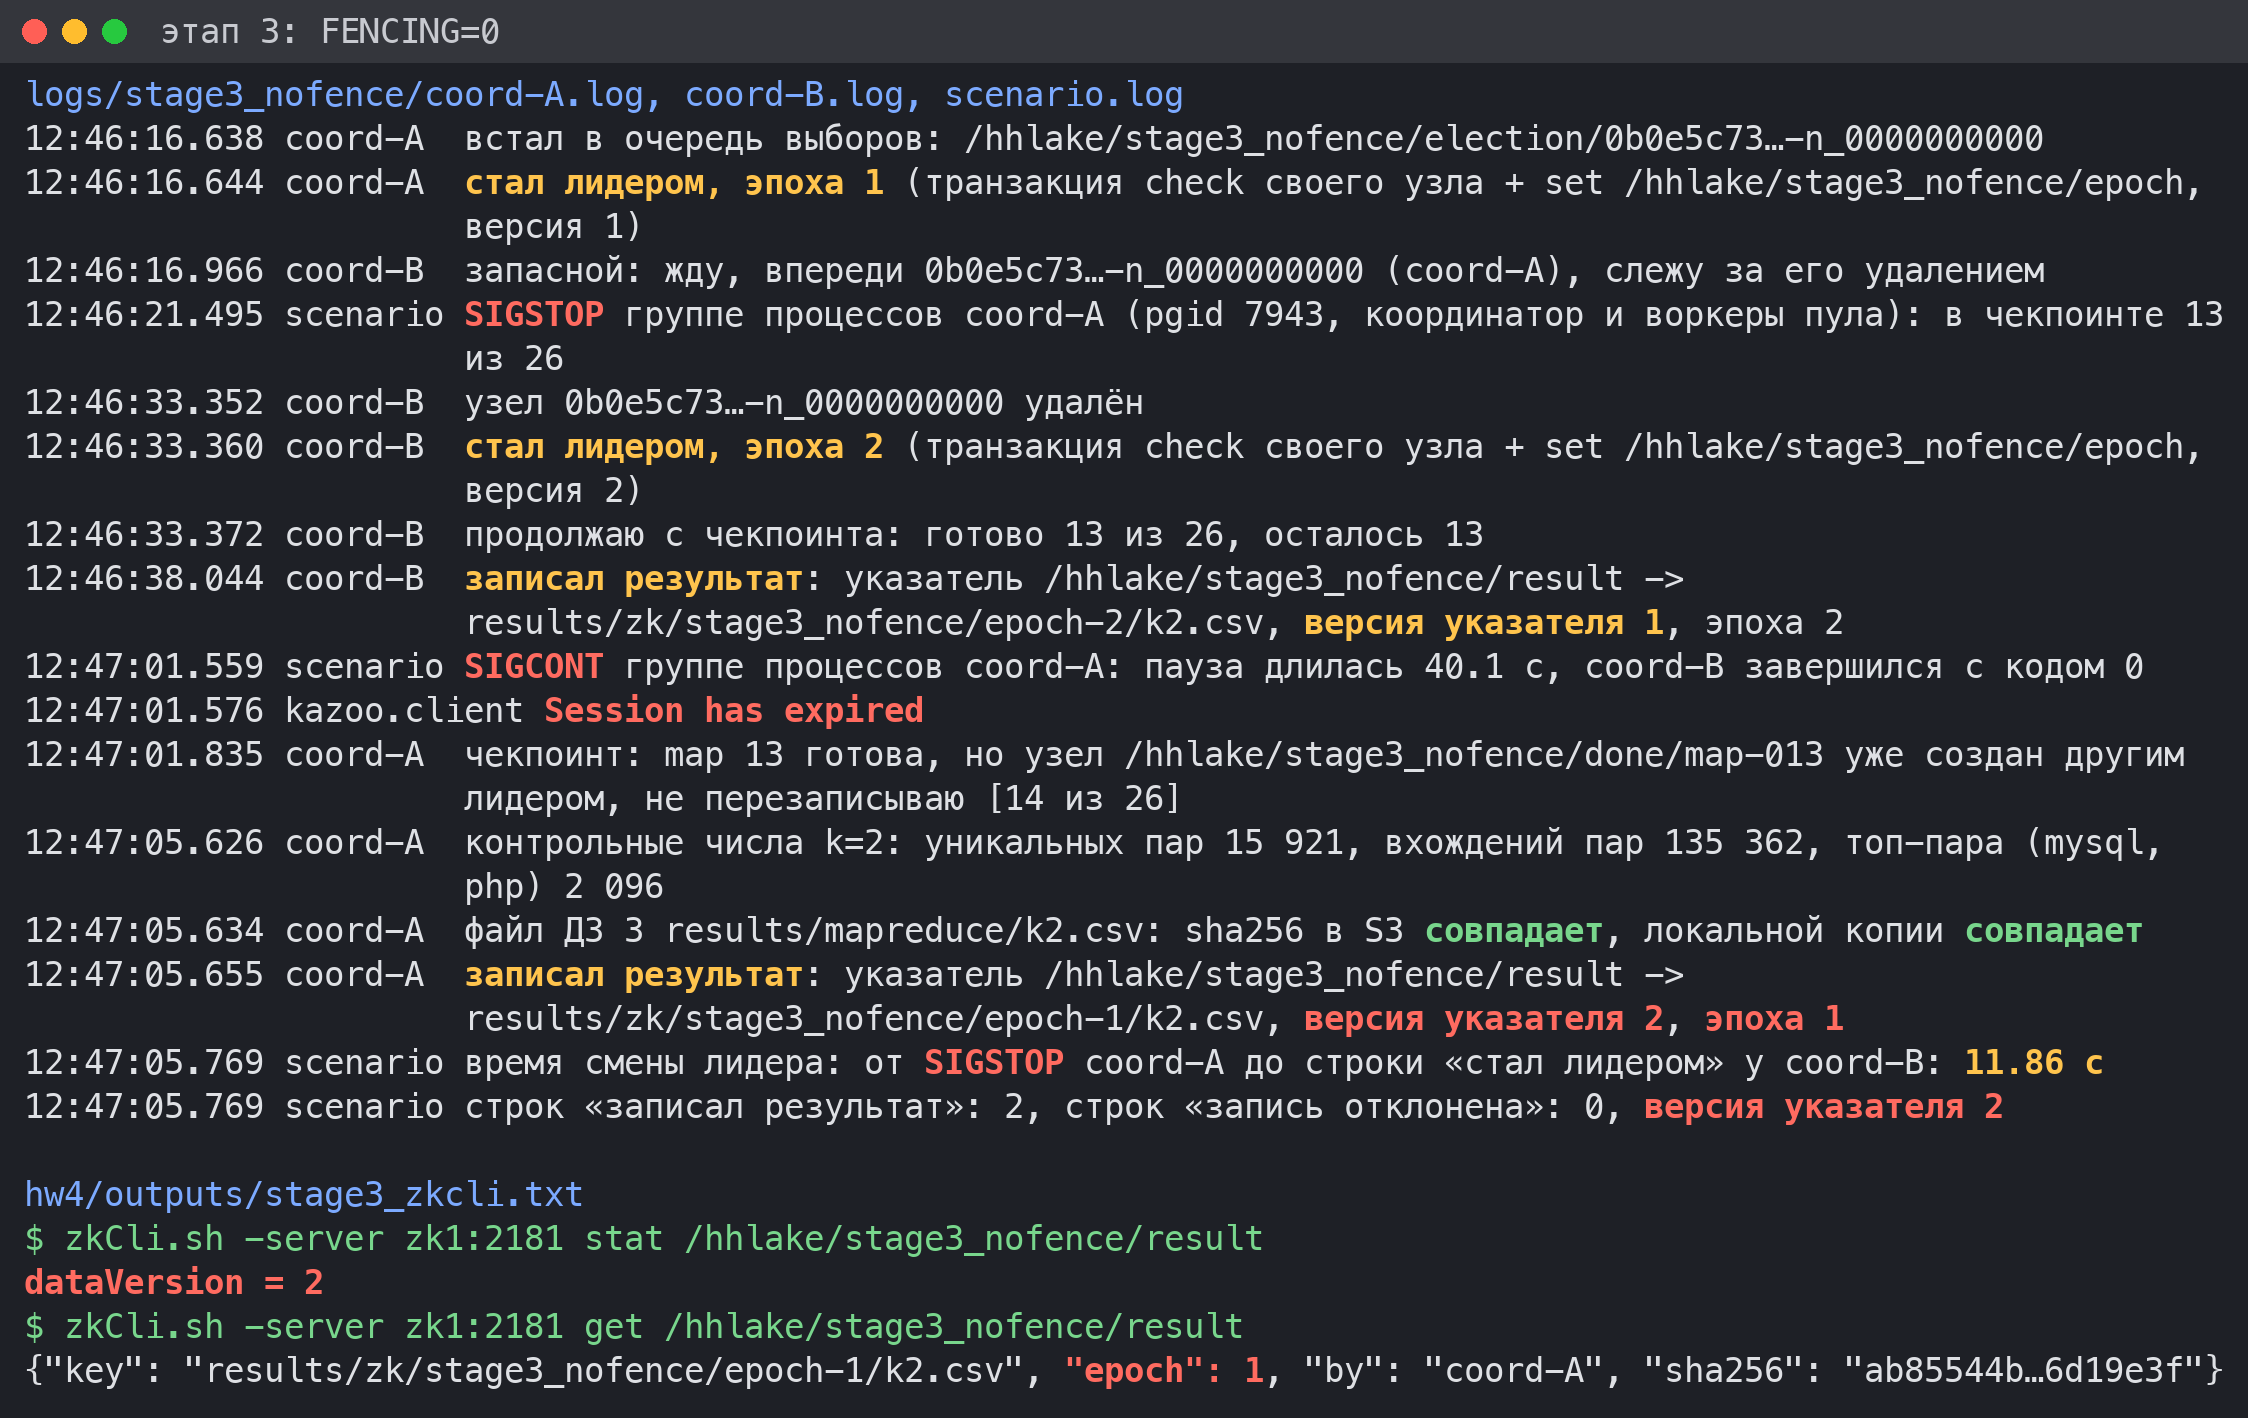
\includegraphics[width=\linewidth]{img/stage3.png}
  \caption{Этап 3: две записи результата, указатель версии 2 от лидера эпохи 1 (фрагмент журналов \code{logs/stage3\_nofence/*.log} и вывода \code{hw4/outputs/stage3\_zkcli.txt}, строки отобраны, uuid и sha256 сокращены)}
  \label{fig:stage3}
\end{figure}

Запасной продолжил с чекпоинта и пересчитал только задачи 13--25. Обе копии сошлись с ДЗ\,3: 15\,921 уникальная пара, 135\,362 вхождения, топ-пара (mysql, php) 2\,096, 229\,388 записей, 5\,382 вакансии варианта. Хеш sha256 итогового CSV (\code{ab85544b\ldots6d19e3f}) совпадает с \code{results/mapreduce/k2.csv} и в S3, и в локальной копии.

После \code{SIGCONT} координатор coord-A не знает, что он больше не лидер. Он досчитал свои задачи 13--25, но узлы чекпоинта для них уже создал coord-B, и coord-A их не перезаписал. Поэтому его reduce прочитал тот же чекпоинт, что и reduce у coord-B: части 0--12 от coord-A и 13--25 от coord-B, а пересчитанные «зомби» части в итог не попали. Файлы совпали именно поэтому. Опасно другое: указатель переписал процесс устаревшей эпохи. В журналах \textbf{две} строки «записал результат», у указателя \code{dataVersion = 2}, и он ведёт на файл эпохи 1 от coord-A. Если бы за время паузы кто-то опубликовал более свежий результат, например следующий запуск на новых данных, проснувшийся «зомби» молча затёр бы его. Строки журналов и состояние указателя --- на рис.~\ref{fig:stage3}.


\section{Этап 4: то же с FENCING=1}

Сценарий тот же, запуск \code{FENCING=1 uv run python -m hhlake.zk.scenario}. Лидер сменился за \textbf{12,15\,с}. В 12:47:44.289 coord-B (эпоха 2) записал результат, указатель получил версию 1. В 12:48:07.240 сценарий разбудил coord-A. Тот досчитал, сошёлся с ДЗ\,3 и в 12:48:11.490 пришёл с транзакцией \code{check(epoch, version=1)}, а версия \code{epoch} уже 2. Транзакция отклонена целиком с \code{BadVersionError}, и coord-A удалил свой неопубликованный файл \code{epoch-1/k2.csv}. Строка «записал результат» одна. Команда \code{stat} для указателя показывает \code{dataVersion = 1}, а \code{get} --- ключ \code{epoch-2/k2.csv} от coord-B. В \code{results/zk/stage4\_fence/} лежит один файл. Контрольные числа и sha256 у обеих копий снова совпали с ДЗ\,3 (рис.~\ref{fig:stage4}).

\begin{figure}[H]
  \centering
  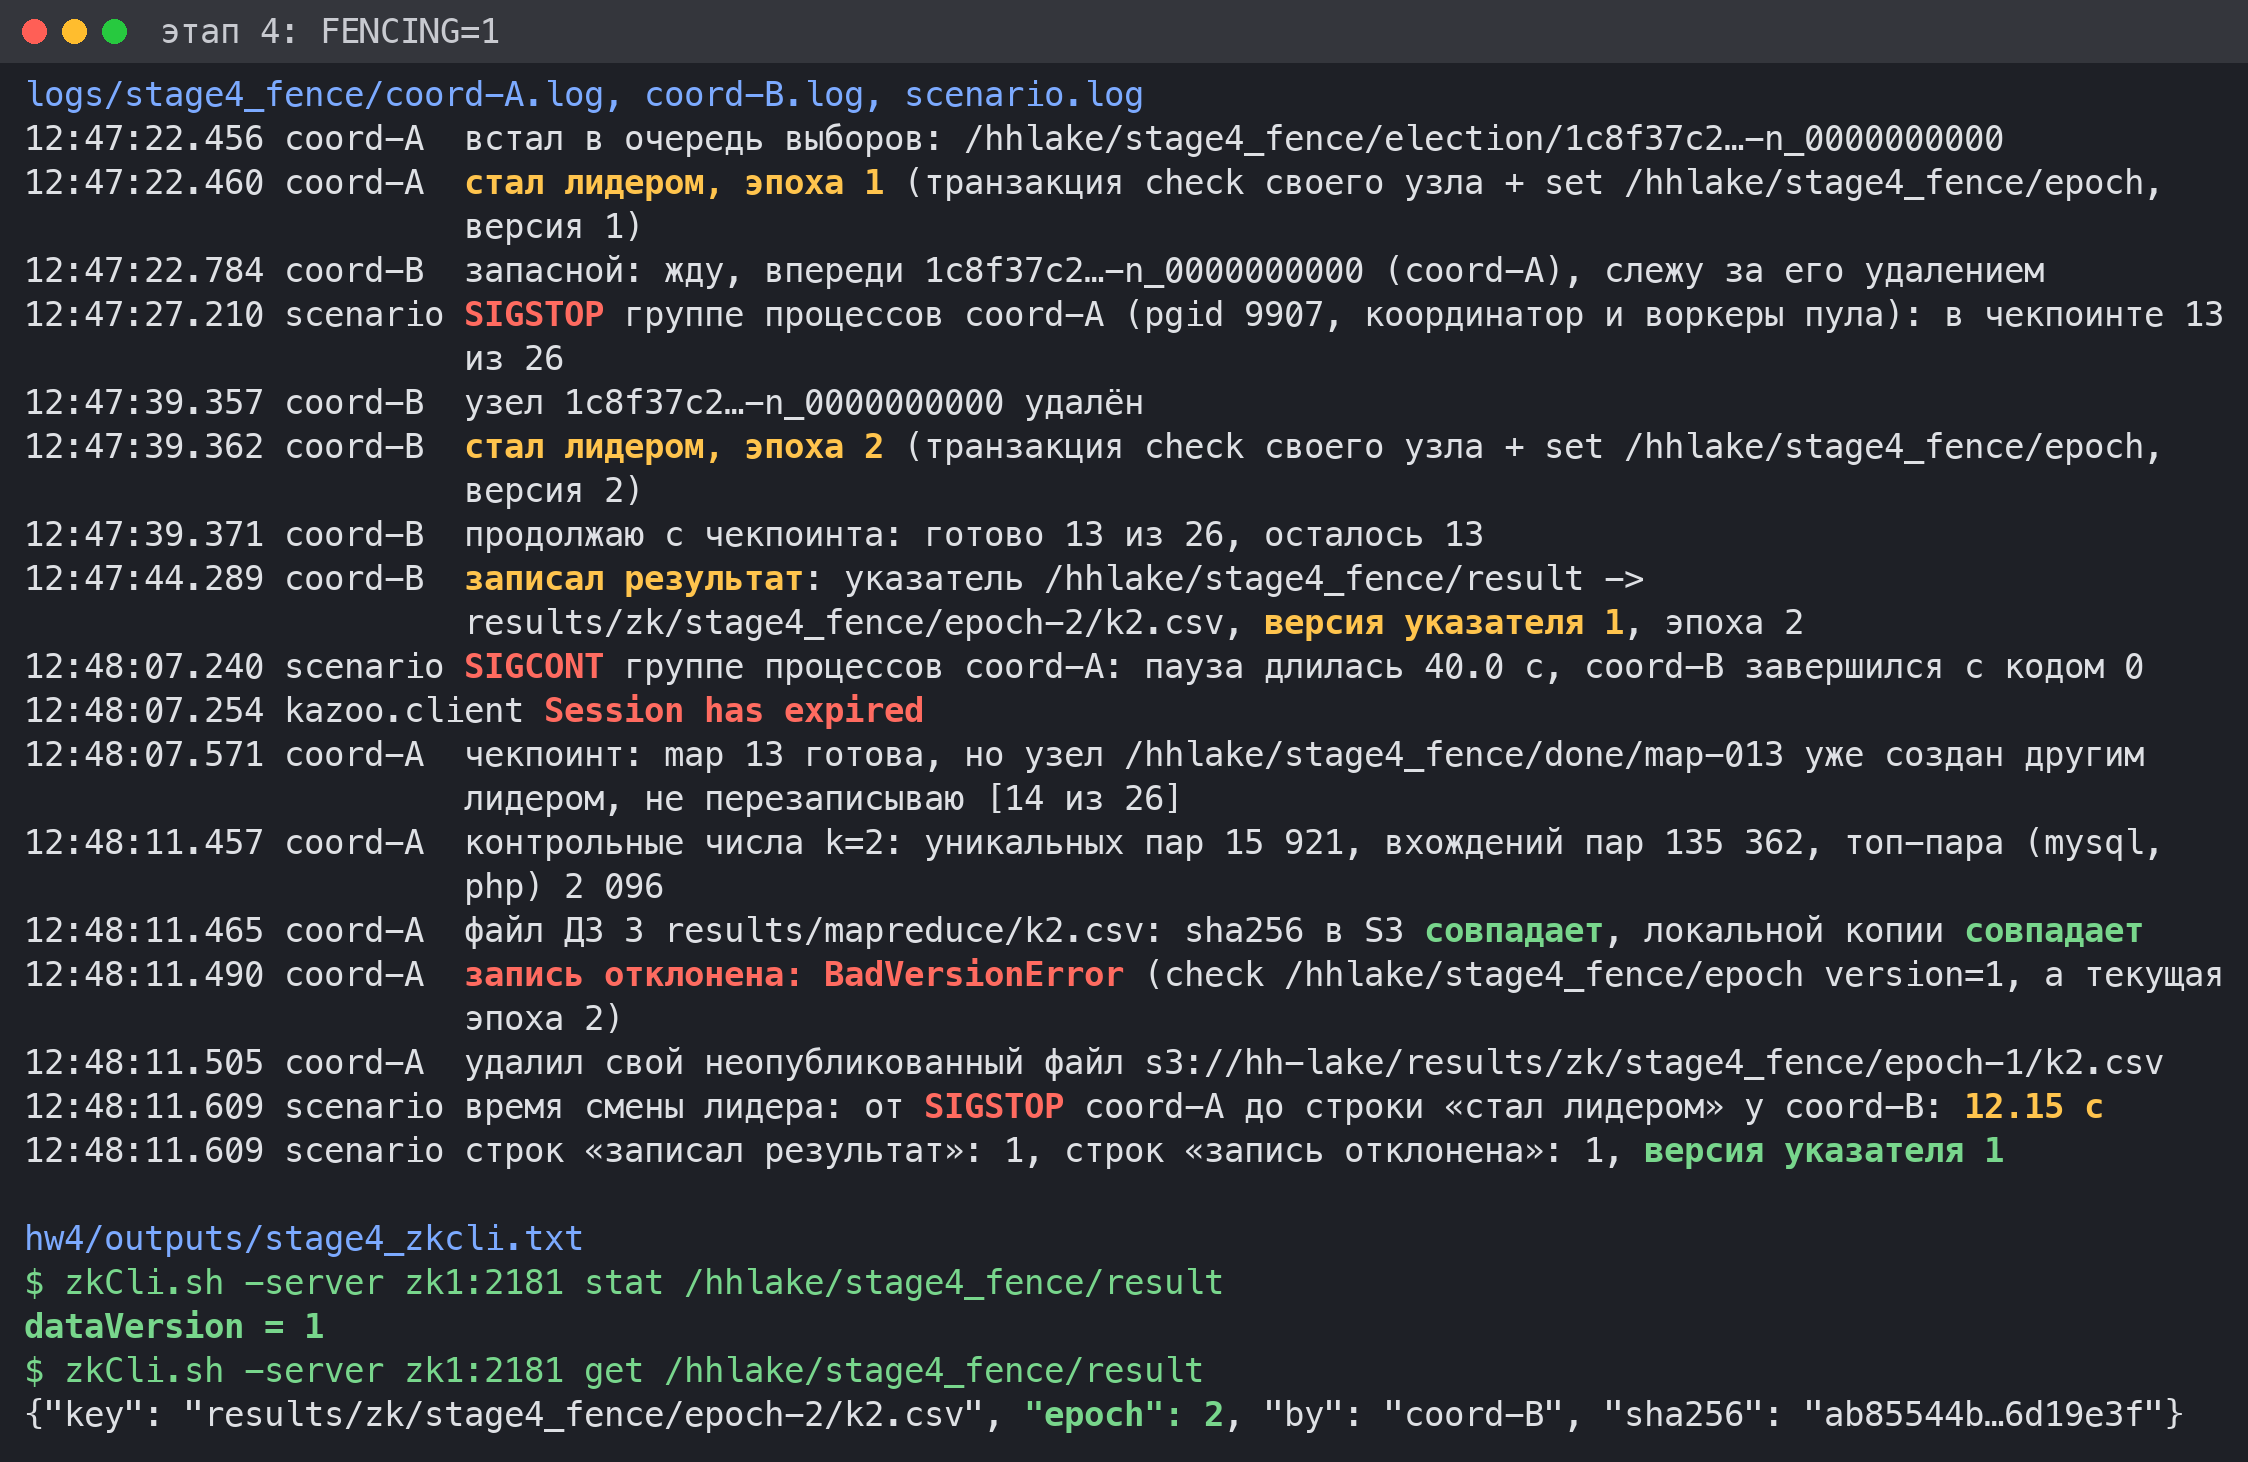
\includegraphics[width=\linewidth]{img/stage4.png}
  \caption{Этап 4: запись старого лидера отклонена, указатель версии 1 от запасного (фрагмент журналов \code{logs/stage4\_fence/*.log} и вывода \code{hw4/outputs/stage4\_zkcli.txt}, строки отобраны, uuid и sha256 сокращены)}
  \label{fig:stage4}
\end{figure}

\section{Ответы на вопросы}

\textbf{Почему серверов три, а не два и не четыре.} ZooKeeper работает, пока живо строгое большинство серверов: так два кворума всегда пересекаются, и у ансамбля не может появиться двух лидеров. Для двух серверов большинство --- оба. Значит, отказ любого из них останавливает систему: два сервера переживают ноль отказов и надёжны хуже одного, ведь сломаться может любой из двух. Три сервера переживают один отказ. Я это проверил: без одного ансамбль работал, без двух --- нет. Четыре сервера тоже переживают только один отказ, потому что большинство из четырёх --- три. Четвёртая машина запаса не даёт, зато каждая запись ждёт подтверждения от трёх серверов, а не от двух. Поэтому ансамбль делают нечётным: 3, 5, 7.

\textbf{Почему эпоху проверяет получатель записи, а не ZooKeeper.} Здесь ZooKeeper выступает службой сессий и выборов. Он замечает, что сессия старого лидера истекла, удаляет его узел и даёт выбрать нового, но остановить замороженный процесс не может. Тот проснётся когда угодно и продолжит с того места, где замер. Перепроверка «я ещё лидер?» перед записью тоже не спасает: пауза может случиться между проверкой и самой записью. Поэтому вместе с записью едет номер эпохи --- токен, то есть число, которое растёт при каждой смене лидера. Сравнить его с последним виденным может только тот, кто принимает запись, и только атомарно с самой записью. В моей работе получатель записи --- узел \code{result} в том же ZooKeeper, и сервер проверяет эпоху транзакцией \code{check(epoch)} + \code{set(result)}. Это роль получателя записи, а не службы выборов: так же условие проверяла бы любая база. Файл в S3 эпоху не проверяет, и в этапе 4 «зомби» свой файл положил (S3 его принял), а после отказа указателя сам удалил. Вреда от этого нет: у каждой эпохи свой ключ \code{epoch-N}, а результатом считается только то, на что ведёт указатель. Если бы результат писался в общий ключ S3 или в таблицу БД, токен должен был бы проверять сам S3 (условный PUT) или БД (\code{UPDATE ... WHERE epoch <= :token}).

\section{Итог}

Ансамбль из трёх серверов ZooKeeper 3.9.6 работает без одного сервера и перестаёт обслуживать запросы без двух. Эфемерный узел живёт, пока жива сессия его владельца. Запасной координатор стал лидером через 11,86 и 12,15\,с после остановки основного и продолжил расчёт с чекпоинта. Результат в обоих запусках совпал с ДЗ\,3 до байта. Без защиты проснувшийся «зомби» перезаписал указатель (две записи, версия 2). С проверкой эпохи на стороне получателя его запись отклонена с \code{BadVersionError}, и указатель остался от запасного (версия 1).

\end{document}
